\documentclass[
	a4paper, % Paper size, use either a4paper or letterpaper
	10pt, % Default font size, can also use 11pt or 12pt, although this is not recommended
	unnumberedsections, % Comment to enable section numbering
	twoside, % Two side traditional mode where headers and footers change between odd and even pages, comment this option to make them fixed
]{t0003}

\usepackage{xcolor}
\newcommand{\blue}[1]{\textcolor{blue}{#1}}
\newcommand{\gray}[1]{\textcolor{gray}{#1}}

\runninghead{Natural Language Models for Data Visualization} % A shortened article title to appear in the running head, leave this command empty for no running head

\setcounter{page}{1} % The page number of the first page, set this to a higher number if the article is to be part of an issue or larger work

%----------------------------------------------------------------------------------------
%	TITLE SECTION
%----------------------------------------------------------------------------------------

\title{Natural Language Models for Data Visualization\\ Utilizing nvBench Dataset} % Article title, use manual lines breaks (\\) to beautify the layout

\author{
	Shuo Wang and Carlos Crespo-Quinones
}

\date{\footnotesize DATASCI 266: Natural Language Processing \\ UC Berkeley School of Information \\ \{shuo.wang, carlos.d.crespo\}@ischool.berkeley.edu}

% Full-width abstract
\renewcommand{\maketitlehookd}{%
	\begin{abstract}
		\noindent Translation of natural language into syntactically correct commands for data visualization is an important application of natural language models and could be leveraged to many different tasks. A closely related effort is the task of translating natural languages into sql queries, which in turn could be translated into visualization with additional information from the natural language query supplied\cite{Zhong:2017qr}. In order to contribute to the progress in this area of research, we built natural language translation models to construct simplified versions of data and visualization queries in a syntax called Vega Zero first proposed by Luo, Yuyu, et al\cite{Luo:2021qr}. In this paper, we explore the design and performance of these sequence to sequence transformer based machine learning architecture using large language models such as BERT as encoders to predict visualization commands from natural language queries. 
	\end{abstract}
}

%----------------------------------------------------------------------------------------

\begin{document}

\maketitle % Output the title section

%----------------------------------------------------------------------------------------
%	ARTICLE CONTENTS
%----------------------------------------------------------------------------------------

\section{Introduction}

Data visualization is an integral part of data analysis and communcation, highly skilled professionals spend significant portion of their working hours constructing data queries and turn them into charts and graphs. The potential application of machine learning models to understand the underlying data and translate natural language queries into data visualization would greatly enhance the efficiency and productivity of many tasks. Not only would such tools enhance our existing ability to understand and communicate our data, it could also help us uncover previously overlooked information.

Some immediate applications include: creating bar, line and scatter plots of sql tables, transform and group data with a table and display the aggregated data and joining and combining tables of data to extract information and display visually.

Previous research in this area has included explorations of transforming natural language into SQL commands\cite{Zhong:2017qr, Yu:2019qr} with deep learning models and natural language to visualization interfaces\cite{Cox:2001qr}. NvBench is a new dataset created to facilitate the research to further integrate the process of natural language to data query and data query to visualizations\cite{Luo:2021qr} . Leveraging this data set and the ncNet transformer model architecture\cite{Luo:2022qr}, we further explore the various modeling possibilty in our work.

In this paper, we have used the nvBench as our train, validation and test dataset to create BERT encoder based multi-head attention transformer models and compare the performance of the new models with the performance of the ncNet model (also a sequence to sequence transformer model). Our goal is to explore the possibility of a generalized natural language to visualization process which the ability of the system to handle natural language inputs is not limited by the input training data. We have provided below the main results of our research and detailed description and analysis of the input data, model architecture and model performance.

From our reseach, the BERT encoder based sequence to sequence transformer model was able to achieve an overall accuracy of 79\%, confirming our hypothesis of the possibility to leverage transferred learning of BERT models to data visualization tasks.

\section{Background}

Natural language to visualization research has been conducted for decades, some of these efforts include early approaches to manually program rule-based logic for the handling of anticipated user inputs in multi-model systems\cite{Cox:2001qr} and more recent attempts to incorporate machine learning and optimization techniques\cite{Aurisano:2016qr}. However these systems are limited in functionality by the ability of the designer of the systems to anticipate the possible inputs from users. What if the user uses a word that the system has never seen? What if the natural language input was written in a idiomatic way that was not anticipated by the training data? These limitations could potentially be addressed with the recent advances in large language models such as BERT and GPT through transfer learning.

Recent research exists for applying BERT model to the task of data visualization\cite{Can:2021qr} by converting natural language into vector representation embeddings and use these embeddings to predict various ingredients needed for the visualization of tabular data such as chart type, data columns and aggregation type. However, the structured approach to the problem inherently limits the expressive power of the system to generate complex visualizations.

A new dataset, nvBench\cite{Luo:2021qr}, was made publicly available for research purposes in 2021. The dataset contains pairs of natural language queries and data visualization commands in vega zero syntax\cite{Luo:2022qr}. A self-contained sequence-to-sequence model, ncNet\cite{Luo:2022qr}, created for and trained on the dataset was also made available. We base our research on this dataset and the ncNet transformer model, modifying the architecture to use BERT and other language models to train and test generalizable natural lanuage to data visualization models. 

\section{Methods}

\subsection{Data}

\subsubsection{nvBench}

The dataset contains 7247 visualization queries (labels). Each query contains visualization type and data retrieval command meant to be run against an underlying database with multiple tables, which contain the actual data to be display. Below is an example of a visualization query:

\begin{quote}
Visualize \blue{BAR} \gray{SELECT JOB\_ID , SUM(MANAGER\_ID) FROM employees WHERE salary BETWEEN 8000 AND 12000 AND commission\_pct != "null" OR department\_id != 40 GROUP BY JOB\_ID ORDER BY JOB\_ID ASC}
\end{quote}

\begin{figure}
	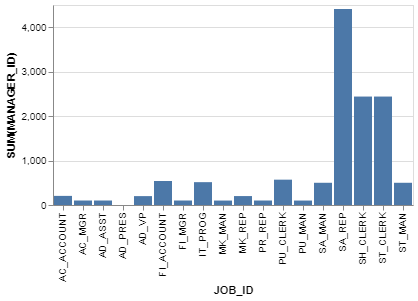
\includegraphics[width=\linewidth]{visualization.png}
	\caption{Rendering: Visualize \blue{BAR} \gray{SELECT JOB\_ID , SUM(MANAGER\_ID) FROM employees WHERE salary BETWEEN 8000 AND 12000 AND commission\_pct != "null" OR department\_id != 40 GROUP BY JOB\_ID ORDER BY JOB\_ID ASC}.}
	\label{fig:visualization}
\end{figure}

In this example, the chart type is ``PIE'', followed by the SQL statement for data retrieval. Figure \ref{fig:visualization} shows the rendering result of the query.

The example visualization query is mapped to several natural language queries, from which we train our models:

\begin{quote}
1. For those employees whose salary is in the range of 8000 and 12000 and commission is not null or department number does not equal to 40, show me about the distribution of job\_id and the sum of manager\_id , and group by attribute job\_id in a bar chart, I want to sort in ascending by the bar.

2. For those employees whose salary is in the range of 8000 and 12000 and commission is not null or department number does not equal to 40, a bar chart shows the distribution of job\_id and the sum of manager\_id , and group by attribute job\_id, and could you order x axis in asc order?
\end{quote}

In total, there are 25762 natural language queries, averaging 3.55 natural langauge queries for every visualization query.

\subsubsection{Augmented Data}

Due to the complexity of SQL syntax, a simplified version of the visualization query is used in place of the original query, called vega zero\cite{Luo:2022qr}:

\begin{quote}
mark \blue{bar} data \blue{employees} encoding x \blue{hire\_date} y aggregate \blue{count hire\_date} transform filter \blue{salary between 8000 and 12000 and commission\_pct != "null" or department\_id != 40} bin x by \blue{month}	
\end{quote}

Where the visualization query is flattened into a sentence with special markers designating locations of information, please refer to \cite{Luo:2022qr} for complete syntax. In our research, we follow the same syntax rules.

Since this syntax only supports single table queries, it is not possible to predict queries where the joining of tables are necessary, so we only train and test our models on a subset of nvBench dataset, with 2988 visualization queries for training, 186 visualization queries for validation and 625 visualization queries for test.

The natural language queries are also augmented to include the template of vega zero queries:

\begin{quote}
\blue{<N>} For those employees whose salary is in the range of 8000 and 12000 and commission is not null or department number does not equal to 40 , draw a line chart about the change of department\_id over hire\_date , display by the X from low to high . \blue{</N>} \blue{<C>} mark \blue{[T]} data employees encoding x  \blue{[X]} y aggregate  \blue{[AggFunction] [Y]} color \blue{[Z]} transform filter \blue{[F]} group \blue{[G]} bin \blue{[B]} sort \blue{[S]} topk \blue{[K] </C> <D>} employees \blue{<COL>} hire\_date salary department\_id last\_name first\_name \blue{</COL> <VAL>} Bull Lex Seo Bell Chen Lee Gee Banda King Baer Fay \blue{</VAL> </D>}
\end{quote}

The natural language query is enclosed in <N> </N> markers, the vega zero template is enclosed in <C> </D> markers and the locations of vega zero query fields are marked by special tokens: [T], [X], [Y], [Z], [F], [G], [B], [S] and [K]. These are the syntax used by the original ncNet sequence to sequence transformer model and we follow the same rules for our models as well.

\subsubsection{Data Loader}

The augmented data were provided in the Github repo for the ncNet paper\cite{Luo:2022qr} , which we use unaltered. However, the original dataloader no longer works the latest version of Pytorch, we rewrote the dataloader to be used for training and testing the ncNet model and our own models.

\subsection{Model}

\subsubsection{ncNet}

\begin{figure*}
	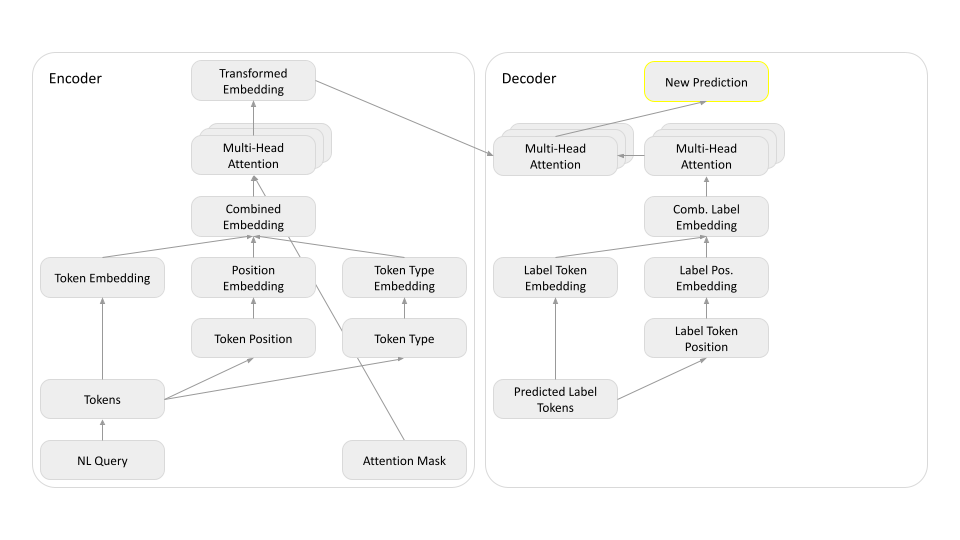
\includegraphics[width=\linewidth]{ncnet_architecture.png}
	\caption{Architecture of ncNet model.}
	\label{fig:ncnet}
\end{figure*}

The ncNet\cite{Luo:2022qr} model is a sequence to sequence multi-head transformer model, where the encoder transforms the natural language queries into embeddings combining position and token type information, and apply multiple layers of multi-head attention transformers to incorporate contextual information into the encoded embeddings. Shown in Figure  \ref{fig:ncnet},  The decoder then takes in the encoded embeddings and the embeddings of the previously predicted tokens to further transform the predicted tokens with attention to the encoded embeddings. We us the ncNet model as our baseline, and replace the encoder with various different architectures.

One important fact to note is that the ncNet model uses all words occuring in the training, testing and validation dataset as vocabulary. Therefore letting the possibility of natural language query inputs.

We also remove the attention mask (referred to as attention forcing in Luo 2022\cite{Luo:2022qr}) used in ncNet to create another baseline for our experiments, since attention mask are not applicable to our models.

\subsubsection{BERT Model}

\begin{figure*}
	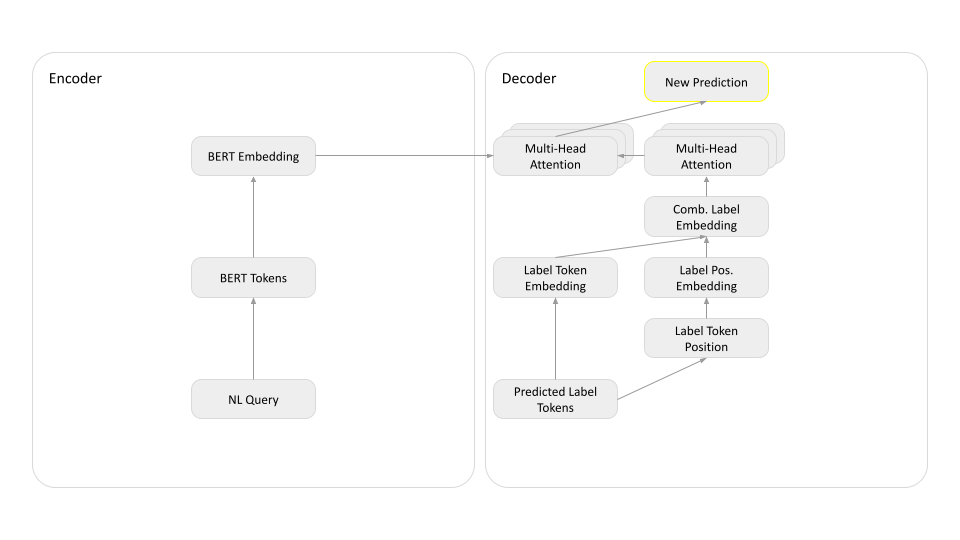
\includegraphics[width=\linewidth]{ncbert_architecture.png}
	\caption{Architecture of ncBERT model.}
	\label{fig:ncbert}
\end{figure*}

\begin{figure*}
	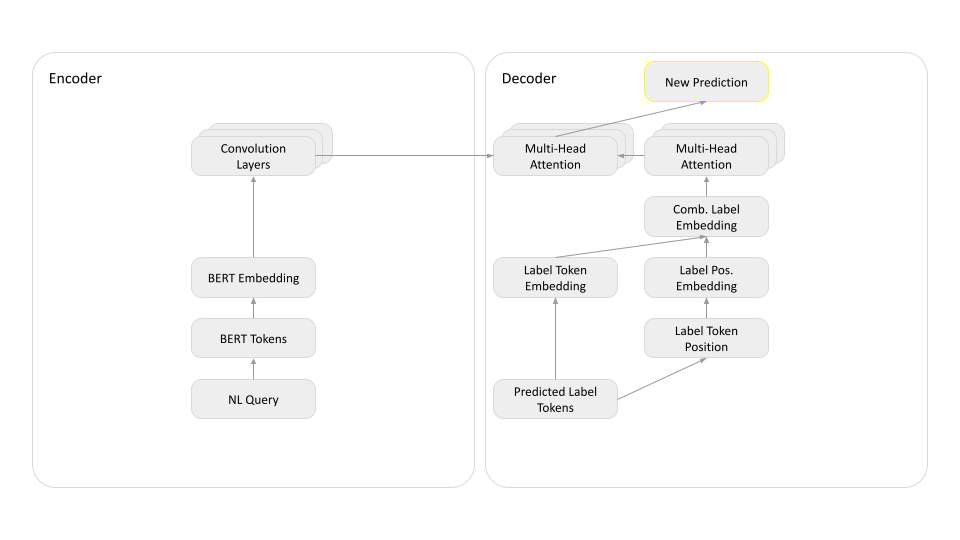
\includegraphics[width=\linewidth]{ncbert_cnn_architecture.png}
	\caption{Architecture of ncBERT\_CNN model.}
	\label{fig:ncbertcnn}
\end{figure*}

We then proceed to replace the ncNet encoder with the BERT model encoder, as shown in Figure \ref{fig:ncbert}. Because the BERT model is pre-trained with a much larger vocabulary, the hope is that this knowledge would transfer to the new model, ncBERT, once we fine tune it. We train an additional BERT encoder model with convolutional layers added to the BERT embeddings, in order to distill relevant information from BERT model embeddings before decoding, as the BERT embedding has a much larger dimension that may contain information irrelevant to the data visualization task. The convolutional layers incorporated model is shown in Figure \ref{fig:ncbertcnn} .

\subsubsection{Combining ncNet and BERT Model}

\begin{figure*}
	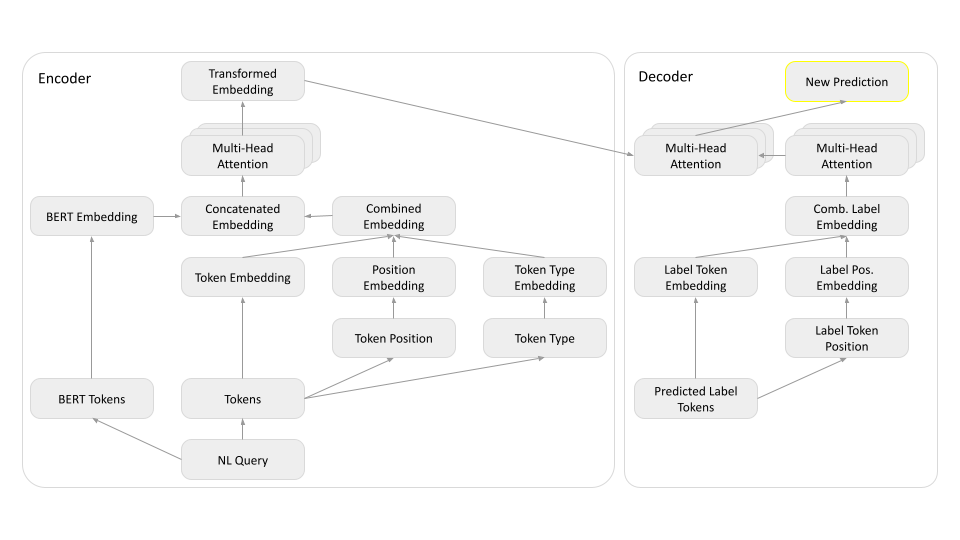
\includegraphics[width=\linewidth]{ncnetbert_architecture.png}
	\caption{Architecture of ncNetBERT model.}
	\label{fig:ncnetbert}
\end{figure*}

Finally, we create an encoder combining both the ncNet and BERT encoders, we achieve this by reshaping the embeddings from BERT to the same dimension as ncNet encoder and concatenating them together. The architecture of the model can be found in Figure \ref{fig:ncnetbert}. The motivation of creating this model is to analyze the effect of BERT embedding on the baseline model and explore the potential of enhancing the original encoder without completely replacing it. However, the implication of this approach is that words that does not exist in the original ncNet encoder still could not be used, further research needs to be done to remove this limitation. 

\subsection{Evaluation}

The models are trained and tested with training dataset of size 25238, validation dataset of size 1430 and test dataset of size 4920. Each model is run over at least 5 epochs with a learning rate of 0.0005 and the resulting losses are recorded.

Then the accuracy of the models are evaluated by running predictions with the models over the test dataset, with the natural language query tokens and the first n-1 tokens of the label as input (the label tokens are masked so that successive predictions of label are not affected by future label tokens), counting the total number of correct predictions and dividing it by the total number of predictions.

Finally, we evaluate the models one more time with a guide search algoirthm to prediction. The algorithm starts the prediction with the start of sentence token, then repeatedly predicts the next label token with guidance until the end of sentence token is reached. This evaluation provides a more realistic measure of the model's usability. The accuracy from this evaluation is defined as the total number of complete label match over the total number of test labels.

\section{Results}

\section{Discussion}

%----------------------------------------------------------------------------------------
%	 REFERENCES
%----------------------------------------------------------------------------------------

\phantomsection
\bibliographystyle{unsrt}
\bibliography{t0003.bib}

%----------------------------------------------------------------------------------------

\end{document}
